%% Contrôle recto-verso, deux compétences (Nommer un angle, sommet et côtés).
%% Recto : Nommer un angle ; verso : Sommet et côtés d'un angle.
%% Réunit les anciens contrôles par compétence (un par face).
%% POUR LE CORRIGÉ : remplacer \corrigefalse par \corrigetrue (dans \begin{document}).

%% Font size %%
\documentclass[11pt]{article}

%% Load the custom package
\usepackage{Mathdoc}
\usepackage{colortbl}
\usetikzlibrary{angles,calc}

%% Numéro de séquence %% Titre de la séquence %%
\renewcommand{\centerhead}{S04 - Éval : Nommer un angle, sommet et côtés}

%% Spacing commands %%
\renewcommand{\baselinestretch}{1} \setlength{\parindent}{0pt}

% =================== Recto : Nommer un angle ===================
% Corrigé : la feuille est écrite une seule fois (\feuille).
\newif\ifcorrige
% Réponse (en mode math) : pointillés dans le sujet, réponse en rouge dans le corrigé
% \rep[largeur]{réponse}
\newcommand{\rep}[2][1.6cm]{\makebox[#1]{$\vphantom{\widehat{A}}$\ifcorrige\textcolor{red}{$#2$}\else\dotfill\fi}}
% Réponse rédigée (texte) sur une ligne : \ligne{réponse}
\newcommand{\ligne}[1]{\makebox[\linewidth][l]{\rule{0pt}{3ex}\ifcorrige\textcolor{red}{#1}\else\dotfill\fi}}
% Nom à entourer dans le corrigé : \entoure[r]{nom} (r = bonne réponse)
\newcommand{\entoure}[2][]{\def\coulcadre{white}\ifcorrige\if r#1\def\coulcadre{red}\fi\fi\tikz[baseline=(m.base)]\node[draw=\coulcadre,thick,rounded corners=2mm,inner sep=1.5pt](m){#2};}
% Nom déjà entouré (exemple fait, en noir)
\newcommand{\entourenoir}[1]{\tikz[baseline=(m.base)]\node[draw,thick,rounded corners=2mm,inner sep=1.5pt](m){#1};}

% ---- Macros de dessin (reprises du QCM DS-6C04-05) ----
% Triangle XYZ avec l'angle de sommet X grisé.
% \triangleMarque[échelle]{X}{Y}{Z}{x_X,y_X}{x_Y,y_Y}{x_Z,y_Z}
\newcommand{\triangleMarque}[7][0.75]{%
  \begin{tikzpicture}[scale=#1]
    \coordinate (P1) at (#5); \coordinate (P2) at (#6); \coordinate (P3) at (#7);
    \coordinate (G) at ($1/3*(P1)+1/3*(P2)+1/3*(P3)$);
    \begin{scope}
      \clip (P1) -- (P2) -- (P3) -- cycle;
      \fill[gray!45] (P1) circle (5mm);
      \draw[thick] (P1) circle (5mm);
    \end{scope}
    \draw[thick] (P1) -- (P2) -- (P3) -- cycle;
    \node at ($(P1)!-4mm!(G)$) {$#2$};
    \node at ($(P2)!-4mm!(G)$) {$#3$};
    \node at ($(P3)!-4mm!(G)$) {$#4$};
  \end{tikzpicture}%
}

% Angle de sommet V, de mesure #2 degrés, premier côté orienté à #3 degrés.
% \angleDessin[échelle]{mesure}{rotation}{L1}{V}{L2}
\newcommand{\angleDessin}[6][1]{%
  \begin{tikzpicture}[scale=#1]
    \coordinate (V) at (0,0);
    \coordinate (P) at (#3:1.8); \coordinate (Q) at ({#3+#2}:1.8);
    \draw[gray!70!black, fill=gray!30] (0,0) -- (#3:4.5mm)
      arc[start angle=#3, delta angle=#2, radius=4.5mm] -- cycle;
    \draw[thick] (P) -- (V) -- (Q);
    \fill (P) circle (1pt); \fill (Q) circle (1pt);
    \node at (#3:2.1) {$#4$};
    \node at ({#3+#2/2+180}:5mm) {$#5$};
    \node at ({#3+#2}:2.1) {$#6$};
  \end{tikzpicture}%
}

% Angle grisé avec plusieurs points sur les côtés.
% \anglePoints{dir. côté 1}{dir. côté 2}{sommet}{pt 1 côté 1}{pt 2 côté 1}{pt 1 côté 2}{pt 2 côté 2}
% (laisser {} si un point est absent ; dir. côté 1 < dir. côté 2)
\newcommand{\anglePoints}[7]{%
  \begin{tikzpicture}[scale=0.7]
    \draw[gray!70!black, fill=gray!30] (0,0) -- (#1:4.5mm)
      arc[start angle=#1, end angle=#2, radius=4.5mm] -- cycle;
    \draw[thick] (#1:3.2) -- (0,0) -- (#2:3.2);
    \node at ({(#1+#2)/2+180}:3.5mm) {$#3$};
    \fill (#1:1.3) circle (2pt); \node at ($(#1:1.3)+({#1-90}:3.5mm)$) {$#4$};
    \if\relax\detokenize{#5}\relax\else
      \fill (#1:2.6) circle (2pt); \node at ($(#1:2.6)+({#1-90}:3.5mm)$) {$#5$};\fi
    \fill (#2:1.5) circle (2pt); \node at ($(#2:1.5)+({#2+90}:4mm)$) {$#6$};
    \if\relax\detokenize{#7}\relax\else
      \fill (#2:2.7) circle (2pt); \node at ($(#2:2.7)+({#2+90}:4mm)$) {$#7$};\fi
  \end{tikzpicture}%
}

% Angle numéroté (grisé) : \marque{P}{V}{Q}{numéro}{rayon}  (de [VP) vers [VQ), sens direct)
\newcommand{\marque}[5]{\pic[draw, fill=gray!30, angle radius=#5, pic text={\small$#4$}, angle eccentricity=0.65]{angle=#1--#2--#3};}
% Arc à tracer par l'élève : rouge dans le corrigé, rien dans le sujet
\newcommand{\arcrouge}[3]{\ifcorrige\pic[draw=red, very thick, angle radius=8mm]{angle=#1--#2--#3};\fi}

% =================== Verso : Sommet et côtés d'un angle ===================
% (macros renommées avec le suffixe B quand le nom existait déjà au recto :
%  \repB, \entoureB)
% Corrigé : la feuille est écrite une seule fois (\feuille).
% Réponse (en mode math) dans une case de largeur fixe : \repB[largeur]{réponse}
% (pointillés sur le sujet, réponse en rouge sur le corrigé, même place)
\newcommand{\repB}[2][0.8cm]{\makebox[#1]{\ifcorrige\textcolor{red}{$#2$}\else\dotfill\fi}}
% Écriture à entourer : \entoureB{faux} ou \entoureB[r]{bonne réponse}
\newcommand{\entoureB}[2][]{\def\coulcadre{white}\ifcorrige\if r#1\def\coulcadre{red}\fi\fi\tikz[baseline=(m.base)]\node[draw=\coulcadre,thick,rounded corners=2mm,inner sep=2pt](m){#2};}
% Écriture entourée en noir (exemple déjà fait)
\newcommand{\entoureex}[1]{\tikz[baseline=(m.base)]\node[draw=black,thick,rounded corners=2mm,inner sep=2pt](m){#1};}
% Notation d'un angle
\newcommand{\ang}[1]{\widehat{#1}}

% Triangle XYZ dont les côtés sont prolongés (droites fines) ;
% dans le corrigé, les côtés de l'angle de sommet #1 sont repassés en rouge.
% #7, #8, #9 : direction (en degrés) de chaque étiquette par rapport à son sommet.
% \triangleCotes{X}{Y}{Z}{x_X,y_X}{x_Y,y_Y}{x_Z,y_Z}{dir_X}{dir_Y}{dir_Z}
\newcommand{\triangleCotes}[9]{%
  \begin{tikzpicture}[scale=0.62]
    \coordinate (P1) at (#4); \coordinate (P2) at (#5); \coordinate (P3) at (#6);
    \draw[gray] ($(P1)!-0.35!(P2)$) -- ($(P2)!-0.35!(P1)$);
    \draw[gray] ($(P2)!-0.35!(P3)$) -- ($(P3)!-0.35!(P2)$);
    \draw[gray] ($(P3)!-0.35!(P1)$) -- ($(P1)!-0.35!(P3)$);
    \draw[thick] (P1) -- (P2) -- (P3) -- cycle;
    \ifcorrige
      \draw[red, line width=1.6pt] ($(P2)!-0.35!(P1)$) -- (P1) -- ($(P3)!-0.35!(P1)$);
    \fi
    \node at ($(P1)+(#7:4.5mm)$) {$#1$};
    \node at ($(P2)+(#8:4.5mm)$) {$#2$};
    \node at ($(P3)+(#9:4.5mm)$) {$#3$};
  \end{tikzpicture}%
}

% Trois demi-droites de même origine T passant par F, G, D ;
% dans le corrigé, les côtés de l'angle GTD sont repassés en rouge.
\newcommand{\eventail}{%
  \begin{tikzpicture}[scale=0.62]
    \coordinate (T) at (0,0);
    \coordinate (F) at (10:2.2); \coordinate (G) at (85:1.9); \coordinate (D) at (150:2.0);
    \draw[thick] (T) -- (10:3.5); \draw[thick] (T) -- (85:3.0); \draw[thick] (T) -- (150:3.1);
    \ifcorrige
      \draw[red, line width=1.6pt] (85:3.0) -- (T) -- (150:3.1);
    \fi
    \foreach \p in {F,G,D} \draw (\p) ++(-2pt,-2pt) -- ++(4pt,4pt) ++(-4pt,0) -- ++(4pt,-4pt);
    \node at ($(F)+(-80:4mm)$) {$F$};
    \node at ($(G)+(-5:4mm)$) {$G$};
    \node at ($(D)+(240:4mm)$) {$D$};
    \node at (-90:3.5mm) {$T$};
  \end{tikzpicture}%
}

% Bandeau de compétence en tête de chaque face
\newcommand{\bandeau}[3][]{\noindent\colorbox{gray!15}{\parbox{\dimexpr\linewidth-2\fboxsep}{\textbf{Compétence #2 : #3}\hfill\textit{\small #1}}}\par}

\newcommand{\feuille}{%
\phantom{0}
\vspace{-.5cm}

\entetedevoirs{40}
\enlargethispage{8mm}

\vspace{-2mm}
{\small\competences{
6C04-GEO10 & Nommer un angle & & & & \\ \hline
6C04-GEO11 & Sommet et côtés d'un angle & & & & \\ \hline
}}

\smallskip
\begin{center}
\textit{Durée : 35 minutes \quad -- \quad Total : 40 points \quad -- \quad Calculatrice non autorisée.}
\end{center}

\vspace{-3mm}
\bandeau[]{6C04-GEO10}{Nommer un angle}
\vspace{-0.5cm}
\begin{exercicedevoir}[5][Nomme l'angle grisé]
\vspace{-0.3cm}
Écris le nom de l'angle grisé, comme dans l'exemple.

\renewcommand{\arraystretch}{1}
\begin{tabularx}{\textwidth}{@{}*{6}{>{\centering\arraybackslash}X}@{}}
\triangleMarque[0.5]{U}{V}{W}{0,0}{3.4,0}{2.4,2} &
\triangleMarque[0.5]{B}{C}{D}{3,2.2}{0,0}{3.4,0.2} &
\triangleMarque[0.5]{F}{E}{G}{0,2.2}{0.4,0}{3.4,1.4} &
\triangleMarque[0.5]{R}{P}{Q}{3.2,1.2}{0,0}{0.8,2.4} &
\triangleMarque[0.5]{J}{K}{I}{1.4,0}{0,2.2}{3.4,1.8} &
\triangleMarque[0.5]{Z}{Y}{X}{0,1.8}{2.4,0}{3.4,2.4} \\
\textit{Ex.} : $\widehat{VUW}$ & a) \rep{\widehat{CBD}} & b) \rep{\widehat{EFG}} & c) \rep{\widehat{PRQ}} & d) \rep{\widehat{KJI}} & e) \rep{\widehat{YZX}} \\
\end{tabularx}
\end{exercicedevoir}

\vspace{-0.85cm}
\begin{exercicedevoir}[5][Plusieurs angles dans une figure]
\vspace{-0.3cm}
\begin{minipage}[c]{0.4\linewidth}\centering
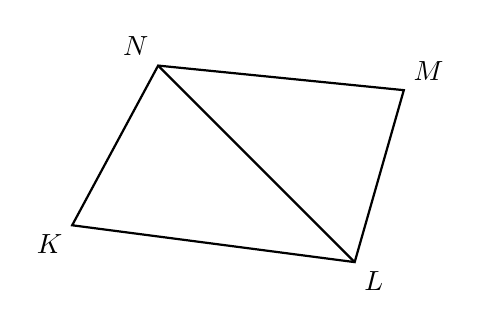
\begin{tikzpicture}[scale=0.78]
  \coordinate (K) at (0,0.6); \coordinate (L) at (4.6,0);
  \coordinate (M) at (5.4,2.8); \coordinate (N) at (1.4,3.2);
  \marque{L}{K}{N}{1}{6mm}
  \marque{N}{M}{L}{2}{6mm}
  \marque{N}{L}{K}{3}{9mm}
  \marque{L}{N}{M}{4}{9mm}
  \arcrouge{K}{N}{L}
  \arcrouge{M}{L}{N}
  \draw[thick] (K) -- (L) -- (M) -- (N) -- cycle;
  \draw[thick] (L) -- (N);
  \node[below left] at (K) {$K$}; \node[below right] at (L) {$L$};
  \node[above right] at (M) {$M$}; \node[above left] at (N) {$N$};
\end{tikzpicture}
\end{minipage}\hfill
\begin{minipage}[c]{0.57\linewidth}
\textbf{a.} Nomme chaque angle numéroté, comme dans l'exemple.

\smallskip
\textit{Ex.} : angle 1 : $\widehat{LKN}$ \qquad angle 2 : \rep{\widehat{LMN}}

\smallskip
angle 3 : \rep{\widehat{KLN}} \qquad angle 4 : \rep{\widehat{LNM}}

\medskip
\textbf{b.} Sur la figure, repasse d'un \textbf{arc de couleur}\newline
l'angle $\widehat{KNL}$, puis l'angle $\widehat{NLM}$.
\end{minipage}
\end{exercicedevoir}

\vspace{-0.85cm}
\begin{exercicedevoir}[4][Entoure les bons noms]
\vspace{-0.3cm}
Pour chaque angle grisé, entoure les \textbf{deux} noms corrects, comme dans l'exemple.

\renewcommand{\arraystretch}{1.3}
\begin{tabularx}{\textwidth}{@{}*{3}{>{\centering\arraybackslash}X}@{}}
\angleDessin[0.6]{60}{10}{P}{Q}{R} &
\angleDessin[0.6]{65}{120}{I}{G}{H} &
\angleDessin[0.6]{50}{200}{D}{U}{V} \\
\textit{Ex.} : \entourenoir{$\widehat{PQR}$}\,\entoure{$\widehat{QPR}$}\,\entourenoir{$\widehat{RQP}$}\,\entoure{$\widehat{PRQ}$} &
a) \entoure{$\widehat{GIH}$}\,\entoure[r]{$\widehat{IGH}$}\,\entoure[r]{$\widehat{HGI}$}\,\entoure{$\widehat{GHI}$} &
b) \entoure{$\widehat{UDV}$}\,\entoure{$\widehat{DVU}$}\,\entoure[r]{$\widehat{VUD}$}\,\entoure[r]{$\widehat{DUV}$} \\
\end{tabularx}
\end{exercicedevoir}

\vspace{-0.85cm}
\begin{exercicedevoir}[6][Un angle, plusieurs noms]
\vspace{-0.3cm}
\begin{minipage}[c]{0.28\linewidth}\centering
\anglePoints{0}{60}{R}{S}{T}{U}{}
\end{minipage}\hfill
\begin{minipage}[c]{0.7\linewidth}
\textbf{a.} Écris \textbf{quatre} noms différents de l'angle grisé.

\smallskip
\rep{\widehat{SRU}} \quad \rep{\widehat{TRU}} \quad \rep{\widehat{URS}} \quad \rep{\widehat{URT}}

\medskip
\textbf{b.} Léo a écrit $\widehat{RSU}$ pour nommer cet angle. Explique son erreur et corrige-la.

\ligne{Le sommet $R$ doit être la lettre du milieu : il fallait écrire $\widehat{SRU}$.}
\ligne{}
\end{minipage}
\end{exercicedevoir}



\newpage
\bandeau[]{6C04-GEO11}{Sommet et côtés d'un angle}
\vspace{-0.5cm}


\begin{exercicedevoir}[3][Trouve le sommet]
\vspace{-0.3cm}
Écris le \textbf{sommet} de chaque angle. \hfill \textit{\small (0,5 point par réponse)}

\renewcommand{\arraystretch}{1.5}
\begin{tabularx}{\textwidth}{@{}XXXX@{}}
\textit{Ex.} $\ang{KLM}$ : \makebox[0.8cm]{$L$} &
a) $\ang{PQR}$ : \repB{Q} &
b) $\ang{HIJ}$ : \repB{I} &
c) $\ang{CAB}$ : \repB{A} \\
 & d) $\ang{YZW}$ : \repB{Z} &
e) $\ang{NMV}$ : \repB{M} &
f) $\ang{XEU}$ : \repB{E} \\
\end{tabularx}
\end{exercicedevoir}

\vspace{-1.1cm}
\begin{exercicedevoir}[5][Complète le tableau]
\vspace{-0.3cm}
\begin{minipage}[c]{0.3\linewidth}
Complète le tableau.

\smallskip
\textbf{Attention :} sur les lignes d et e, c'est le \textbf{nom de l'angle} qu'il faut trouver !

\smallskip
\textit{\small (1 point par ligne)}
\end{minipage}\hfill
\begin{minipage}[c]{0.68\linewidth}
\centering
\renewcommand{\arraystretch}{1.3}
\begin{tabular}{|l|c|c|}
\hline
\multicolumn{1}{|c|}{\textbf{Angle}} & \textbf{Sommet} & \textbf{Côtés} \\ \hline
\rowcolor{gray!15} \textit{Ex.} \ $\ang{XYZ}$ & $Y$ & $[YX)$ \ et \ $[YZ)$ \\ \hline
a) \ $\ang{BCD}$ & \repB{C} & \repB[1.3cm]{[CB)} \ et \ \repB[1.3cm]{[CD)} \\ \hline
b) \ $\ang{STU}$ & \repB{T} & \repB[1.3cm]{[TS)} \ et \ \repB[1.3cm]{[TU)} \\ \hline
c) \ $\ang{FHG}$ & \repB{H} & \repB[1.3cm]{[HF)} \ et \ \repB[1.3cm]{[HG)} \\ \hline
d) \ \repB[3.3cm]{\ang{AEV} \text{ ou } \ang{VEA}} & $E$ & $[EA)$ \ et \ $[EV)$ \\ \hline
e) \ \repB[3.3cm]{\ang{NRP} \text{ ou } \ang{PRN}} & $R$ & $[RN)$ \ et \ $[RP)$ \\ \hline
\end{tabular}
\end{minipage}
\end{exercicedevoir}

\vspace{-1.1cm}
\begin{exercicedevoir}[4][Entoure la bonne écriture]
\vspace{-0.3cm}
a) et b) : entoure \textbf{un côté} de l'angle. \quad c) et d) : entoure \textbf{les deux côtés}. \hfill \textit{\small (1 point par réponse)}

\renewcommand{\arraystretch}{1.25}
\begin{tabular}{@{}l@{\hspace{1.5cm}}l@{}}
\textit{Ex.} $\ang{GOK}$ : \ $[GO)$ \ \entoureex{$[OG)$} \ $[OG]$ \ $[KG)$ & \\
a) $\ang{LMN}$ : \ \entoureB{$[LM)$} \ \entoureB[r]{$[ML)$} \ \entoureB{$[ML]$} \ \entoureB{$[NM)$} &
b) $\ang{UVW}$ : \ \entoureB{$[WV)$} \ \entoureB{$[UW)$} \ \entoureB{$[VW]$} \ \entoureB[r]{$[VW)$} \\
\multicolumn{2}{@{}l@{}}{c) Les côtés de $\ang{CDE}$ : \quad \entoureB{$[CD)$ et $[CE)$} \quad \entoureB{$[DC]$ et $[DE]$} \quad \entoureB[r]{$[DC)$ et $[DE)$}} \\
\multicolumn{2}{@{}l@{}}{d) Les côtés de $\ang{PSQ}$ : \quad \entoureB[r]{$[SP)$ et $[SQ)$} \quad \entoureB{$[PS)$ et $[PQ)$} \quad \entoureB{$[SP)$ et $[QS)$}} \\
\end{tabular}
\end{exercicedevoir}

\vspace{-1.1cm}
\begin{exercicedevoir}[8][Sur une figure]
\vspace{-0.3cm}
Complète, puis repasse en couleur les côtés de l'angle demandé.
\hfill \textit{\small (a, b, d, e : 1,5 point ; c, f : 1 point)}

\begin{minipage}[c]{0.3\linewidth}\centering\eventail\end{minipage}\hfill
\begin{minipage}[c]{0.68\linewidth}
\renewcommand{\arraystretch}{1.35}
\begin{tabular}{@{}l@{}}
a) $\ang{DTF}$ : sommet \repB{T} ; \ côtés \repB[1.3cm]{[TD)} et \repB[1.3cm]{[TF)} \\
b) $\ang{FTG}$ : sommet \repB{T} ; \ côtés \repB[1.3cm]{[TF)} et \repB[1.3cm]{[TG)} \\
c) Repasse en couleur les côtés de l'angle $\ang{GTD}$. \\
\end{tabular}
\end{minipage}

\begin{minipage}[c]{0.3\linewidth}\centering\triangleCotes{G}{B}{K}{3,1.9}{0,0.4}{2.4,-0.3}{320}{95}{300}\end{minipage}\hfill
\begin{minipage}[c]{0.68\linewidth}
\renewcommand{\arraystretch}{1.35}
\begin{tabular}{@{}l@{}}
d) $\ang{GBK}$ : sommet \repB{B} ; \ côtés \repB[1.3cm]{[BG)} et \repB[1.3cm]{[BK)} \\
e) $\ang{BKG}$ : sommet \repB{K} ; \ côtés \repB[1.3cm]{[KB)} et \repB[1.3cm]{[KG)} \\
f) Repasse en couleur les côtés de l'angle $\ang{BGK}$. \\
\end{tabular}
\end{minipage}
\end{exercicedevoir}

\vspace{-0.6cm}
}

\begin{document}

\corrigefalse
\feuille

\end{document}

%%% Local Variables:
%%% mode: LaTeX
%%% TeX-master: t
%%% End:
